\chapter{CONCLUSÕES}
\label{cap:05}
dessa forma é possível analisar as transparências de concorrência e replicação. 
Conforme as informações nas figuras \ref{fig:disponibilidade 10 seeds} e \ref{fig:disponibilidade_5_seeds}, é possível ver a transparência de replicação, onde o mesmo objeto está replicado em varias máquinas diferentes, que são os \ac{seed}, mas a transferência é feita de maneira única. 

No desempenho da velocidade de download do arquivo foi possível notar diferenças com o aumento da quantidade de \ac{seed} conectados, com 5 \ac{seed} a velocidade média obtida foi de 2 MiB/S, representado pela figura \ref{fig:geral_5_seeds}, enquanto com 12 \ac{seed}, foi obtido uma velocidade média de 25 MiB/S, representado pela figura \ref{fig:geral_12_seeds}.

A quantidade de \ac{seed} conectados transmitindo arquivos simultaneamente, mostram que as redes \ac{p2p} são transparentes em concorrência, pois os arquivos compartilhados são transmitidos de diversas máquinas diferentes enquanto no cliente é realizado o download de forma única sem ficar evidente que cada parte do arquivo está sendo transmitido por uma máquina diferente. 

Conclui-se que as redes \ac{p2p} se mantém transparentes em concorrência e replicação, se encaixando em sistemas distribuídos. 
\begin{figure}[!htb]
\centering
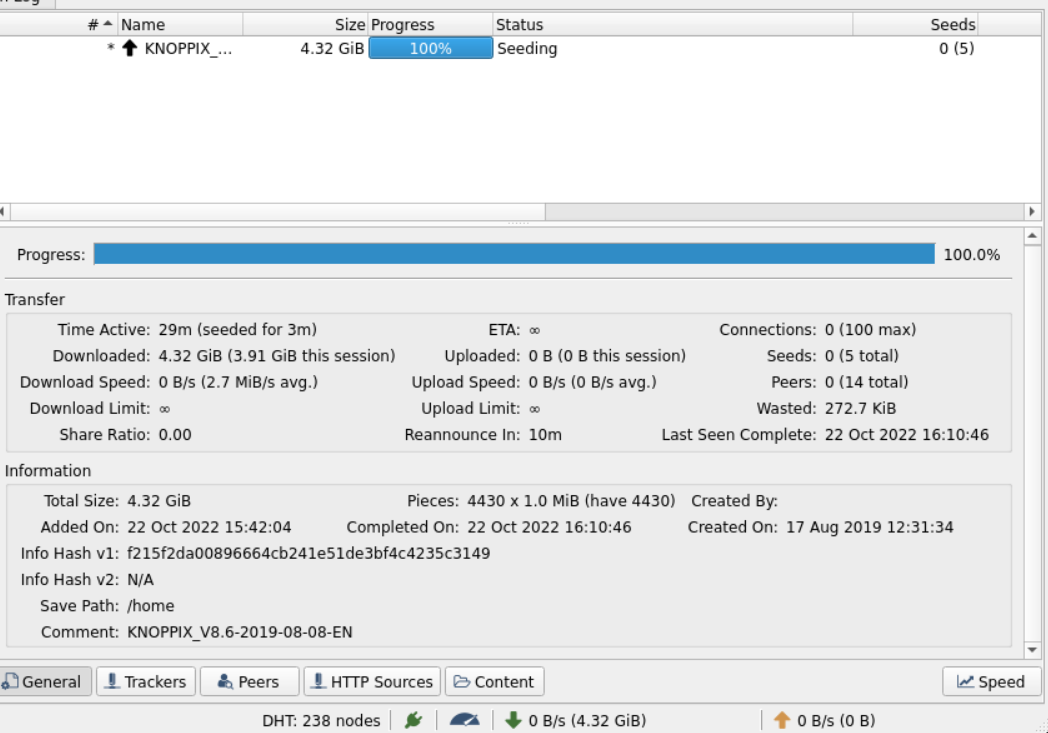
\includegraphics[width=0.7\textwidth]{./images/5 seeds geral.png}
\caption{Informações Gerais de download com 5 seeds}
\label{fig:geral_5_seeds}
\end{figure}

\begin{figure}[!htb]
\centering
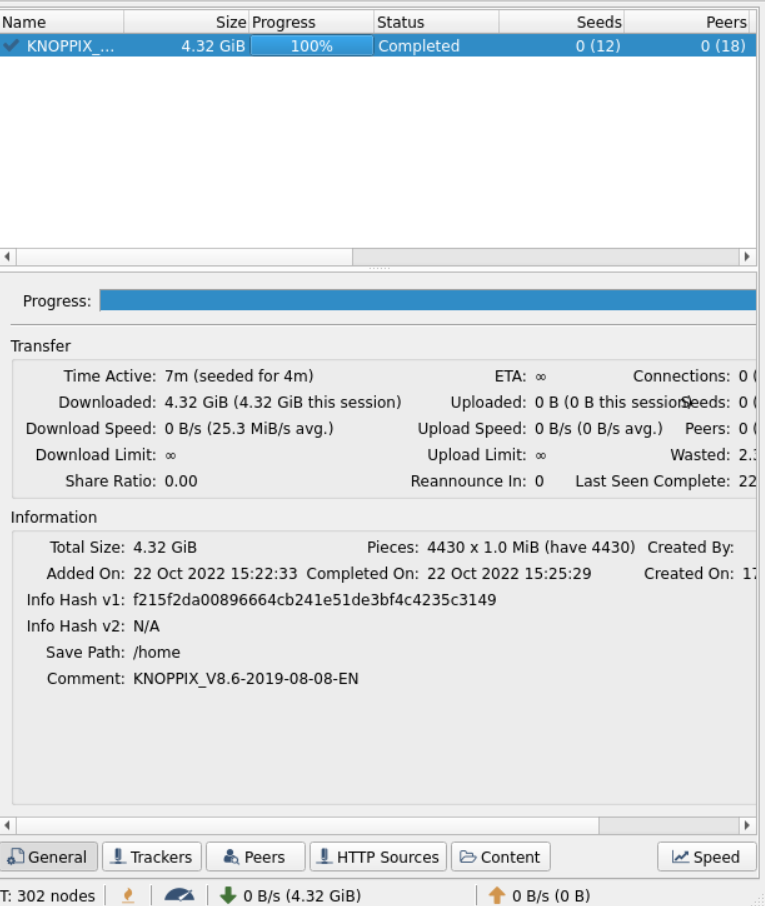
\includegraphics[width=0.7\textwidth]{./images/geral 12 seeds.png}
\caption{Informações Gerais de download com 12 seeds}
\label{fig:geral_12_seeds}
\end{figure}